\documentclass{article}
\usepackage[top=2cm, bottom=2cm, left=2cm, right=2cm]{geometry}
\usepackage[figurename=Figure]{caption}
\usepackage{graphicx} % Required for including pictures
\usepackage{float} % For tables and other floats
\usepackage{amsmath} % For math
\usepackage{amssymb} % For more math
\usepackage{fullpage} % Set margins and place page numbers at bottom center
\usepackage{paralist} % paragraph spacing
\usepackage{listings} % For source code
\usepackage{subfig}   % For subfigures
\usepackage{enumitem} % useful for itemization
\usepackage{circuitikz}
\usepackage{setspace} % to control the linespace
\usepackage{fancyhdr} % for the head and foot of pages
\usepackage{epstopdf}
\usepackage{color}
\definecolor{dkgreen}{rgb}{0,0.6,0}
\definecolor{gray}{rgb}{0.5,0.5,0.5}
\definecolor{mauve}{rgb}{0.58,0,0.82}
\lstset{frame=tb,
  language=Python,
  aboveskip=3mm,
  belowskip=3mm,
  showstringspaces=false,
  columns=flexible,
  basicstyle={\small\ttfamily},
  numbers=left,
  numberstyle=\tiny\color{gray},
  keywordstyle=\color{blue},
  commentstyle=\color{dkgreen},
  stringstyle=\color{mauve},
  breaklines=true,
  breakatwhitespace=true,
  escapeinside=``,
  tabsize=4,
  extendedchars=false 
}

% Set the head and foot of pages
\pagestyle{fancy}
\fancyhf{}
\rhead{120090272}
\chead{DDA2020 Assignment 2}
\lhead{Chuqiao Feng}
\rfoot{Page \thepage}

% The title of homework
\begin{document}
\rmfamily 
\hrule
\begin{center}
	\vspace{.4cm}
	{\textbf { \huge DDA2020 Assignment 2}}
\end{center}
\setlength{\baselineskip}{20pt}
\noindent
{\textbf{Name:} \ Chuqiao Feng \hspace{\fill} \textbf{Due Date:} April 3 2022, 11:59 PM \\ 
{\textbf{Student Number:} \ 120090272 \hspace{\fill} \textbf{Assignment:} Assignment 2 \\
\hrule

% the main problem
\section*{Main: Multiclass classification problem}
\large
\hspace{12pt} In the datasets, the data covers 3 classes, which means we need to solve a multiclass classification problem with support vector machine.
for being recommended to use sklearn.svm.svc() function in python package of sklearn, which only implements only one versus one strategy. So we aggregaate two classes into one and run svc function for three times to find the classifier for data of these three class.
Once we find the SVM model for the datasets, we can predict the label or class of new data by applying data into the model.

% the problem 1
\section*{Problem 1: SVM Model}
The standard SVM model is:\\ $min_{w,b}\quad \frac{1}{2}||w||^2$ \newline \hspace{60pt}$s.t. \quad 1-y_i(w^Tx_i+b)\leq 0, \forall i $\\
Because sklearn package doesn't provide a function with strict separation, so we apply SVM model with slack variables with a large C using C = 1e5.
To construct the solution with sklearn.svm, we define a SVM class where object is the optimal problem mainly as below. 
\begin{lstlisting}
%% the svm problem is a linear seperator, so use C=1e5, lernel="linear"
    svm = SVC(C = C, kernel = "linear")
%% do classification with one vs rest strategy for three times
    for i in range(3):
        Y_new_train = [1 if m == i else -1 for m in self.Y_train]
%% fit the model with svm.fit() function
        svm.fit(self.X_train, Y_new_train)
%% calculate W,b,support_vectors with svm.coef_ and svm.intercept_ and svm.support
        W[i,:] = svm.coef_
        b[i] = svm.intercept_
        support_vectors.append(svm.support_)
%% calculate the error for training data and test data
    train_data_prediction = np.array(list(map(np.argmax, train_cls)))
    test_data_prediction = np.array(list(map(np.argmax, test_cls)))
    train_error = 1 - accuracy_score(train_data_prediction, self.Y_train)
    test_error = 1- accuracy_score(test_data_prediction, self.Y_test)
\end{lstlisting}
As in the result of program, although we set the coefficient for slack variables very large, there are still several points being misclassified of "versicolor" vs rest and "virginica" vs rest. 
So only "setosa" can be linearly separable. \newline
~\\

% the problem 2
\section*{Probelm 2: SVM Model with Slack Variables}
The problem of SVM model with slack variables can be formulated as:\\
$min_{w,b,\epsilon}\quad \frac{1}{2}||w||^2+ C \sum_i^m + \epsilon _i$ \\ \hspace{60pt}$s.t. \quad 1-\epsilon_i-y_i(w^Tx_i+b)\leq 0, \epsilon_i\geq 0, \forall i $\\
In the solution of this optimization problem, if $\alpha_i=0$, the data is correctly classifed and doesn't contribute to the classifier; if $0<\alpha_i<C$, classified correctly on the margin, and corresponding points are support vectors; and if $\alpha_i=C$ and $\epsilon_i>1$, the data is classified incorrectly.
Its lagrange function is: $L(w,b,\alpha)=\frac{1}{2}||w||^2+ C \sum_i^m + \epsilon _i+\sum_i^m[\alpha _i(1-\epsilon_i-y_i(w^Tx_i+b))-\mu_i\epsilon_i]$, with KKT conditions, we easily calculate that $w=\sum_i^m\alpha_iy_ix_i$ and $b=\frac{1}{|M|}\sum_{j\in M}(y_i-\sum_i^m\alpha_iy_ix_i^Tx_j)$, 
applying the model, we can predict the label or class of new data points.
To solve the problem by sklearn.svm functions, process are the same as the problem 1, except that with small C value.
\begin{lstlisting}
%% the svm problem with small C = 0.1 to 1 
    svm = SVC(C = 0.1 * n, kernel = "linear")
\end{lstlisting} and the plot of error changes with C is shown as below:
\begin{figure}[htbp]
	\centering
	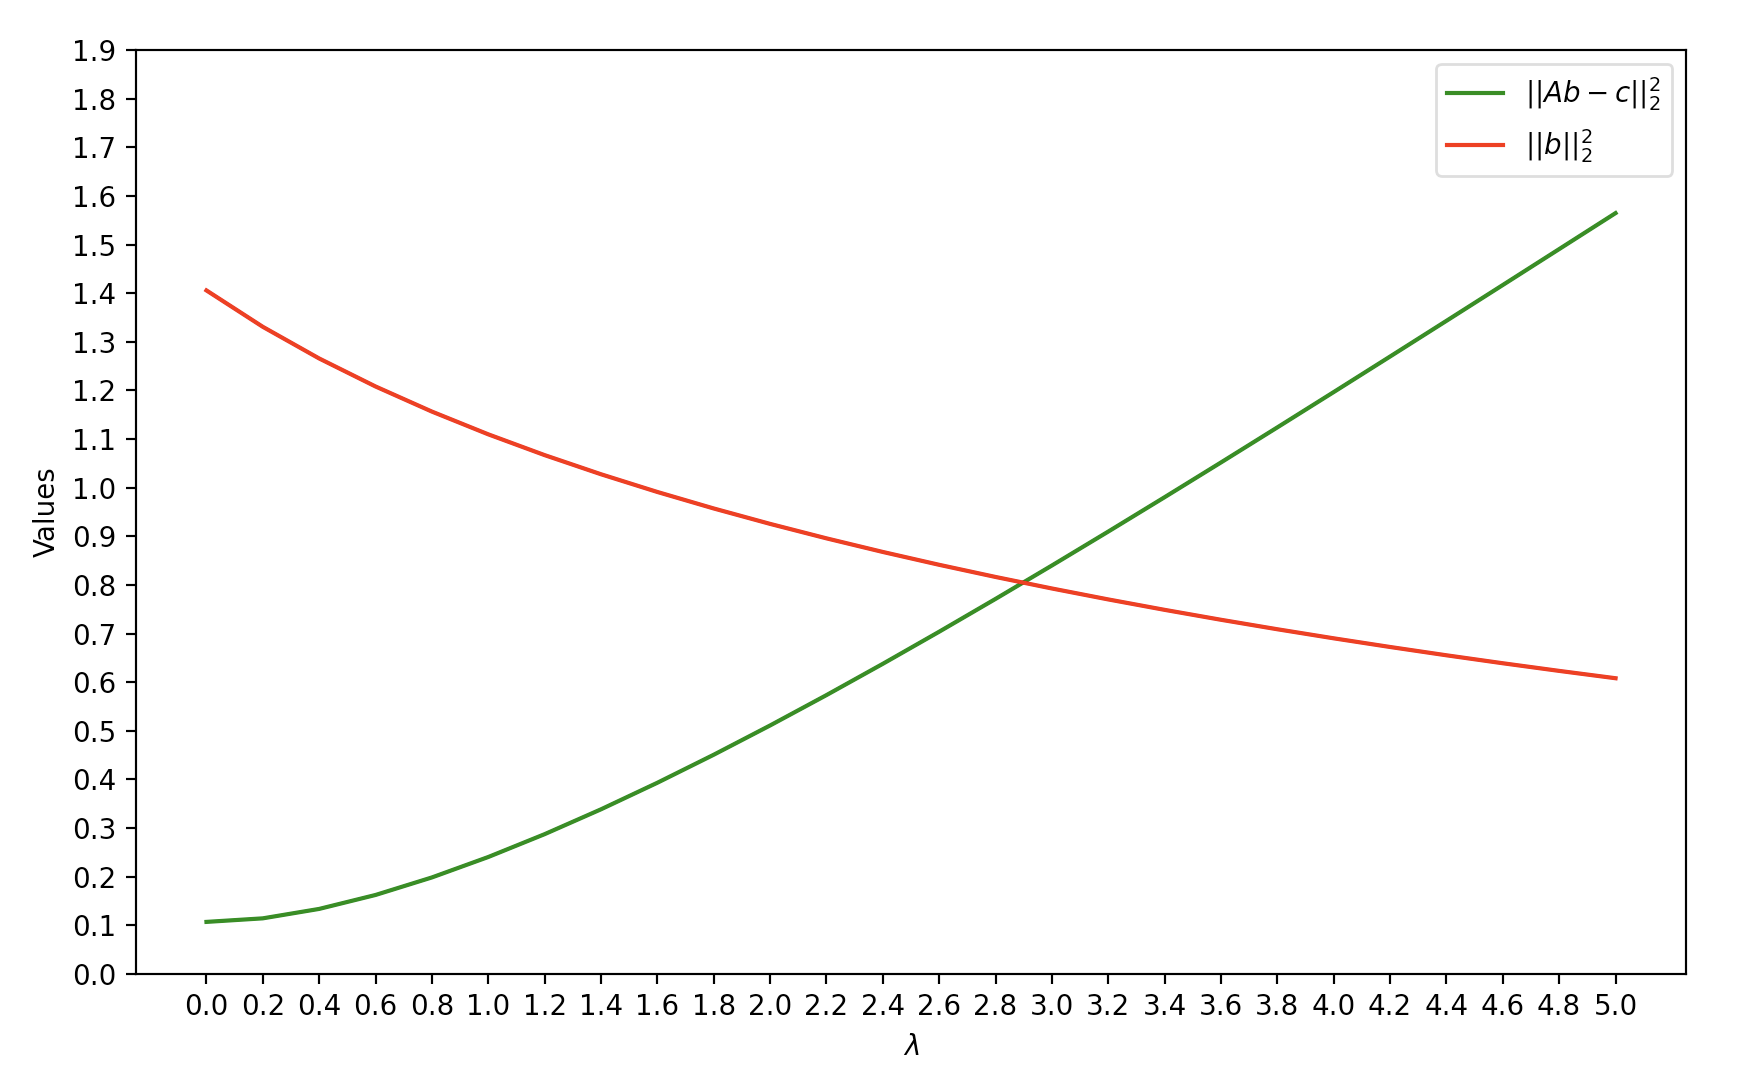
\includegraphics[scale=0.3]{img.jpg}
	\caption{figure of lambda}
	\label{figure}
\end{figure}
% the problem 3
\section*{Problem 3: SVM Model with kernels}
\subsection*{(a) SVM with 2nd-order polynomial kernel}

\subsection*{(b) SVM with 3nd-order polynomial kernel}

\subsection*{(c) SVM with radial basis function kernel}

\subsection*{(d) SVM with sigmoidal kernel}


\end{document}